\subsection{Handling duplicate connections}

\begin{figure}[htb!]
  \centering
    \subfloat[]{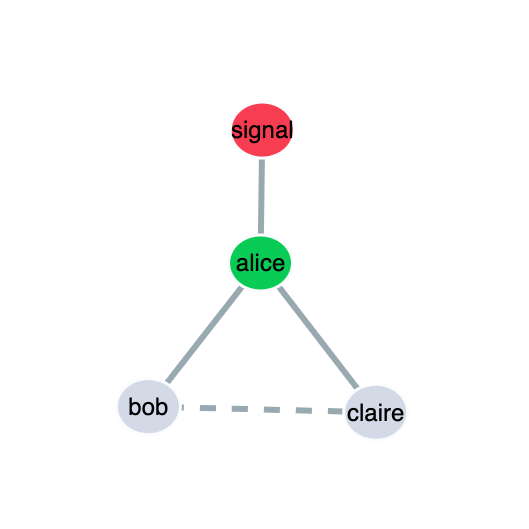
\includegraphics[width=0.25\textwidth]{graphics/analysis/mini-scenarios/double-connection/1.png} \label{fig:filmstrips-double-connections-a}}
    \subfloat[]{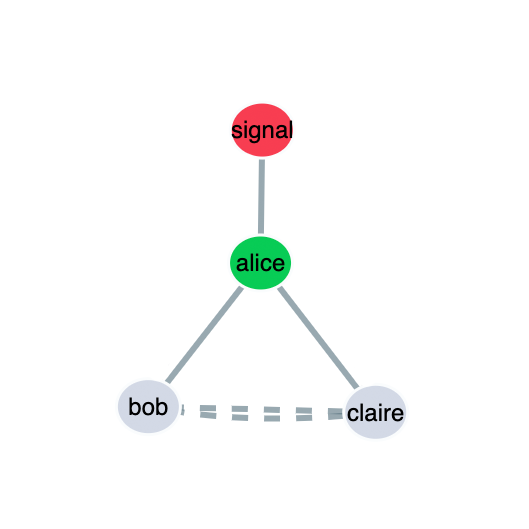
\includegraphics[width=0.25\textwidth]{graphics/analysis/mini-scenarios/double-connection/2.png} \label{fig:filmstrips-double-connections-b}}
	\subfloat[]{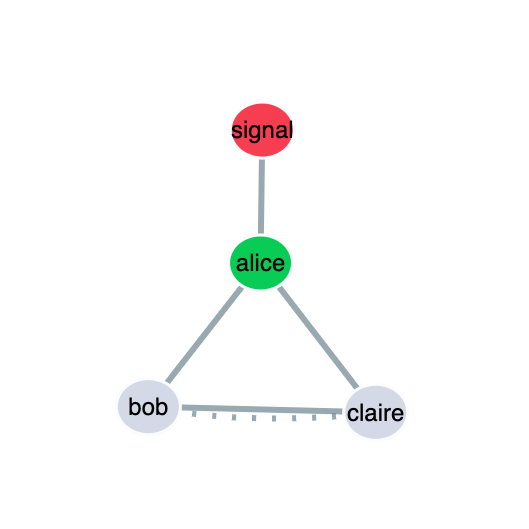
\includegraphics[width=0.25\textwidth]{graphics/analysis/mini-scenarios/double-connection/3.png} \label{fig:filmstrips-double-connections-c}}
	\subfloat[]{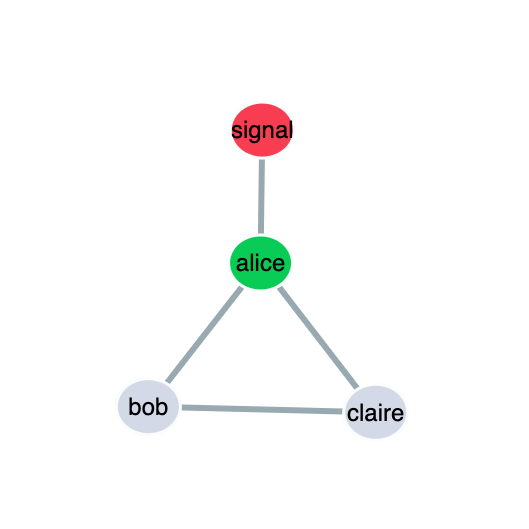
\includegraphics[width=0.25\textwidth]{graphics/analysis/mini-scenarios/double-connection/4.png} \label{fig:filmstrips-double-connections-d}}
	\caption{Both peers want to open a connection}
\label{fig:filmstrips-double-connections}
\end{figure}

Each peer has the restriction that it must have at most one connection to the same peer to save capacity for other peers. However, during the negotiation process it can happen that both peers (\bob \& \claire) try to open a connection to each other at the same time (\vref{fig:filmstrips-double-connections-a}-\vref{fig:filmstrips-double-connections-b}). Both peers are noticing that they have a duplicate connection. Now the issue arises, that both peers want to close the duplicate connection and in the worst case both connections are closed as a result.

This is a known problem from the field of telecommunications. \citet[pp. 194-194]{signaling-systems-book} call this problem \say{Circuit Glare (Dual-Seizure)}.
The Mitosis algorithm solves this problem by applying the fixed rule, that the connection with the lower id will be closed.

Therefore, both peers select the connection with the lowest id and close it (\vref{fig:filmstrips-double-connections-c}). This ensures that one connection will always remain open (\vref{fig:filmstrips-double-connections-d}).